\section{ENCODE data} \label{encode-data-sect}
The Encyclopedia of DNA Elements (ENCODE) project is an international collaboration of research groups with diverse backgrounds and expertise in production and analysis of NGS genomic data.

\emph{Fig. \ref{seq-pic}} shows only some examples of the different platforms and techniques that are used from ENCODE in order to measure diverse biological components.

\begin{figure}[!ht]
\begin{center}
 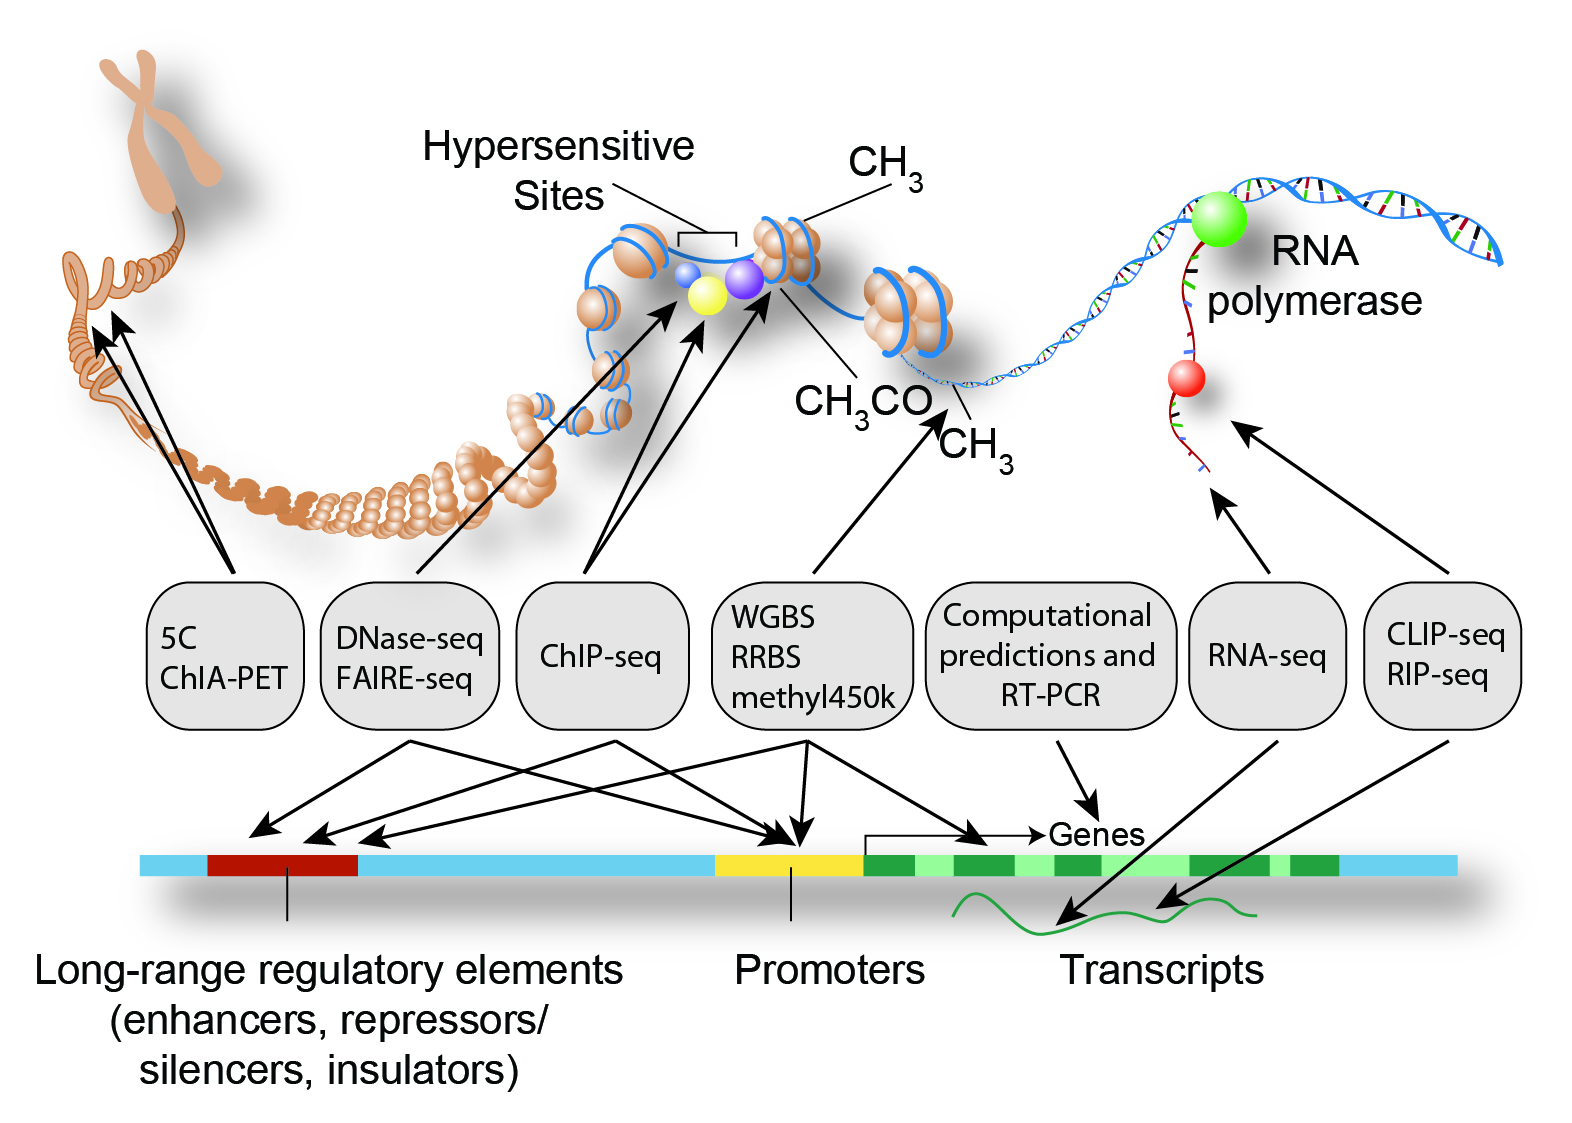
\includegraphics[scale = 0.25]{images/encode-seq.png}
\caption{\emph{Some of the XX-Seq techniques used from the ENCODE projet. Credits: Darryl Leja (NHGRI), Ian Dunham (EBI), Michael Pazin (NHGRI) \citep{Dunham2012}.}}
\label{seq-pic}
\end{center}
\end{figure} 